In order to deal with the risk management, we decided to use the FMECA (Failure Mode, Effects, Criticality, Analysis) Method on the means of production of\moldco company. This means that we consider all the risks related to the operation of the assembly line system.\\

For that purpose, we have, to as a first step, to describe the system. Then we will be able to identify all the threats. After this step, we will identify all the threats that could affects the system and assess them in order to define their criticality.\\
Ultimately, we will see how to compensate these eventual failure modes where appropriate.\\

\subsection{Description of the system}

The assembly line system is composed of two main parts : 
\begin{itemize}
    \item the mechanical system
    \item and the computing's one.\\
\end{itemize}

By the way, we estimate that these two systems are interdependent. In orther words, we have to take into account that if the mechanical part of the assembly line fails, the entire system cannot work anymoer and vice versa.\\
Actually, mechanical part of the production chain can work independently but if the computing system is not working, the mechanical will get problems about its regulation and monitoring.\\

\begin{figure}[h]
    \centering
    \begin{tabular}{| p{4cm} | c | c | c | c | c | c | c | c | c |}
        \hline
        \rowcolor{heading-color}\multicolumn{1}{|c|}{Failure mode} & Failure causes & Failure effect & Detection method & Corrective actions & Severity & Occurrence & Detection & Criticality & RPN\\
        \hline
        Power outage & ? & Stop the production & Beep & Beep & 5 & 1 & 1 & 5 & 5 \\
        \hline
        Noise pollution & Mechanical disruption & Employee's discomfort & Error message & Automatic measurement & 1 & 2 & 2 & 2 & 4 \\
        \hline
        Inherent materiel defect & Obsolescence & Slowdown or stop the production & Error message & Periodic maintenance & 5 & 2 & 1 & 10 & 10 \\
        \hline
        Earthquake & Environment & Stop the production &  &  &  &  &  &  &  \\
        \hline
        Fire & Overheat & Stop the production &  &  &  &  &  &  &  \\
        \hline
        Flood &  & Stop the production &  &  &  &  &  &  &  \\
        \hline
    \end{tabular}
    \caption{FMECA Method}
    \end{figure}

According to the FMECA MEthod, we have to assess two different values in the table of risk.\\

First of all, the Severity (S) which equals to the importance of the consequences that the risk could induce on the production of the factory. More the risk can affect the production line, more the Severity level is high as the following table shows :

\begin{figure}[h]
    \centering
    \begin{tabular}{| p{4cm} | c | c |}
        \hline
        \rowcolor{heading-color}\multicolumn{1}{|c|}{Severity definition} & Severity level & Associated color\\
        \hline
        Insignificant & 1 & green  \\
        \hline
        Minor & 2 & green clair  \\
        \hline
        Significant & 3 & yellow  \\
        \hline
        Serious & 4 & orange  \\
        \hline
        Major & 5 & red  \\
        \hline
    \end{tabular}
    \caption{Table of severity level}
\end{figure}

    Regarding the Occurrence (O), it enables to measure the likelihood of the risk. Mire the risk is potential, more the Occurrence value is high as we can see as below :

    \begin{figure}[h]
        \centering
        \begin{tabular}{| p{4cm} | c | c |}
            \hline
            \rowcolor{heading-color}\multicolumn{1}{|c|}{Occurrence definition} & Occurrence level & Associated color\\
            \hline
            Remote & 1 & green  \\
            \hline
            Very low & 2 & green clair  \\
            \hline
            Low & 3 & yellow  \\
            \hline
            Moderate & 4 & orange  \\
            \hline
            Major & 5 & red  \\
            \hline
        \end{tabular}
        \caption{Table of occurence level}
\end{figure}

Finally, the Detection (D) is measured according to the ease for the operators to discover a failure mode. Higher the value is, easier it is to detect the failure.

\begin{figure}[h]
    \centering
    \begin{tabular}{| p{4cm} | c |}
        \hline
        \rowcolor{heading-color}\multicolumn{1}{|c|}{Detection definition} & Detection level\\
        \hline
        Blatant & 1  \\
        \hline
        Easily identifiable & 2  \\
        \hline
        Discreet & 3  \\
        \hline
        Hard to identify & 4 \\
        \hline
        Very  hard to identify & 5 \\
        \hline
    \end{tabular}
    \caption{Table of detection level}
\end{figure}

Severity, Occurrence and Detection are arbitrarily assessed whereas Criticality and RPN are calculated from these same data.\\

Especially, we have the following relations :
\begin{itemize}
    \item Criticality = Severity \* Occurrence
    \item RPN = Severity \* Occurrence \* Detection = Criticality \* Detection
\end{itemize}

These last two measures enable us to prioritize the risk in order to make the further effort in order to limit them and eventually resolve them if ever they occur.

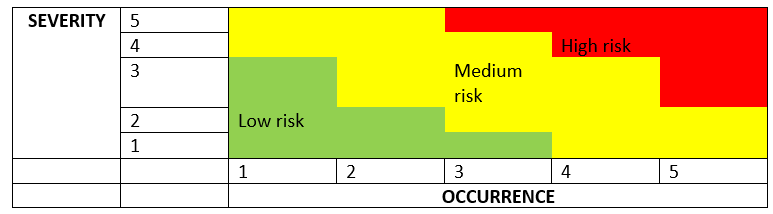
\includegraphics{Img/img-risk.png}

\subsection{Identification of the risks}
\subsubsection{Categorization of the risk}
\subsection{Enhancement of the assembly line function}